% !TEX program = pdflatex
% !TEX encoding = utf8

%%前面那个如果实际操作,完全不含中文可以用pdflatex引擎,注释有utf8没问题,但是正文要小心打出中文符号来。
\documentclass{mcmthesis} %文档类
\usepackage{float} %用于强行定位浮动体,参数H
\mcmsetup{CTeX = false,   % 不使用 CTeX 套装时
        tcn = 0000,  %此为团队码
        problem = A, %问题号
        sheet = true, %
        titleinsheet = true, %
        keywordsinsheet = true,%要关键字
        titlepage = false, %不要这个title
        abstract = true %启用摘要
}

\usepackage{newtxtext} %可以优化数学字体(模板案例也这样来用了)

\title{The \LaTeX{} Template for MCM Version \MCMversion, Preparing!} %标题名称Version \MCMversion



\begin{document} %开始正文

\begin{abstract} %此为摘要环境
    abstract\textbf{ here}  %加粗
     
\begin{keywords} %关键词
    keyword1; keyword2
\end{keywords}

\end{abstract}
\maketitle 

%(这个文档类仍然需要\maketitle)

\section{Section1}

this is sec1


\subsection{assumption}
\subsubsection{add title}

%分开列来强调
\begin{itemize}
	\item A
	\item B
\end{itemize}

%插入一张图片
\begin{figure}[ht]
\centering
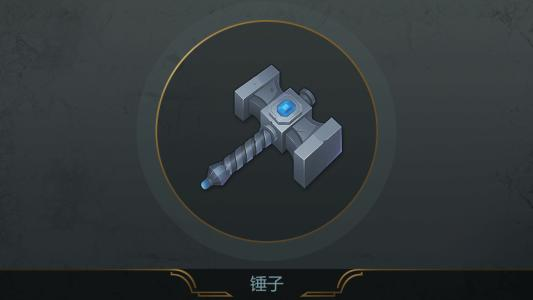
\includegraphics[scale = .35]{/images/hammer.jpg}
\caption{This is a hammer.}
\label{fugure 1}
\end{figure}

%并排插入两张图片
\begin{figure}[htbp]
	\centering
	\begin{minipage}[ht]{0.48\textwidth}
		\centering
		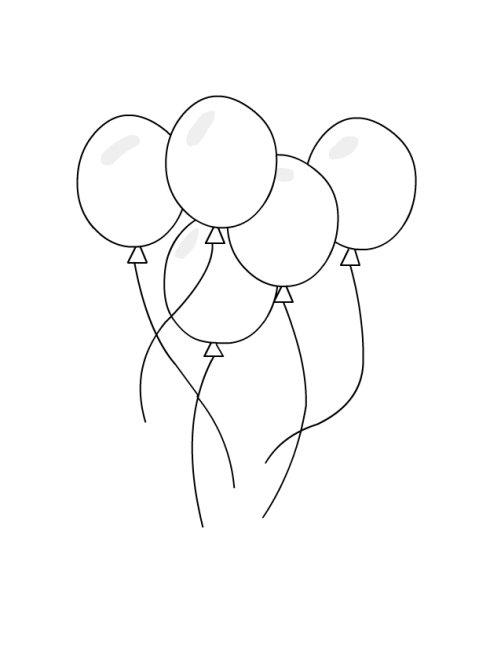
\includegraphics[width=6cm]{/images/ballons}
		\label{fig_22}
		\caption{ballons}
	\end{minipage}
	\begin{minipage}[ht]{0.48\textwidth}
		\centering
		
\includegraphics[width=6cm]{/images/lemon}
		\caption{lemon}
		\label{fig_23}
	\end{minipage}
\end{figure}

\pagebreak  %换页

\begin{align}
	%插入公式
	 \mu =\frac{\partial \eta }{\partial t}  \label{aa}  %编号
\end{align}


${v}_m=\begin{cases}
	
	\sqrt{\left ( 38.9\frac{v}{d} \right )^2 +2400gd}-38.9\frac{v}{d}
	&\text{ if }  d\leq 3mm\\ 
	\frac{d}{0.113+0.845d}
	&\text{ if }  d> \leq 3mm 
\end{cases}$


\begin{table}[ht]
	\caption{Lasting time and effective wave height in the first stage of six geometries}
	\label{Table 1} 
	\begin{tabular}{ccc}
		\hline 
		Geometric shapes & Lasting time(min) & \begin{tabular}[c]{@{}l@{}}Effective wave height in  the firs stage(m)\end{tabular} \\
		\hline
		Cuboid           & about 50min       & >0.2                                                                                  \\
		Cylinder         & Less than 40min   & <0.18                                                                                
	\end{tabular}
\end{table}nd{table}

%写信
\begin{letter}{Dear, Mr. Alpha Chiang}
	
	%信件内容	
	\vspace{\parskip} %空一些行
		Sincerely yours,
		Your friends
	\end{letter}

\begin{thebibliography}{99} %引用部分
    \bibitem{1} D.~E. KNUTH   The \TeX{}book  the American
    Mathematical Society and Addison-Wesley
    Publishing Company , 1984-1986.
    \bibitem{2}Lamport, Leslie,  \LaTeX{}: `` A Document Preparation System '',
    Addison-Wesley Publishing Company, 1986.
    \bibitem{3}\url{https://www.latexstudio.net/}
\end{thebibliography}
    
\begin{appendices} %附录部分
    \section{The prefix(Appendix A) is default}
\end{appendices}

\end{document}